%!TEX root = report.tex
To test if the ratio of autonomous vehicles to human driven vehicles influences the flow of traffic and the number of collisions we run our simulation in batch mode with different initialisations. \Cref{ss:method:experiment:init} presents the different initialisations we use, \cref{ss:method:experiment:measures} discusses what measure, how we measure it en how it relates to real world traffic. 

\subsubsection{Initialisation}
\label{ss:method:experiment:init}
As described in \cref{ss:method:experiment:init} we need to decide on a graph to use and the ratio of human driven vehicles to autonomous cars. 

If one does not take the effect of right-of-way rules or various traffic signs into account there are only two interesting `interactions' between cars, namely two lines of cars that zip merge and lines of cars that intersect each other. \Cref{fig:method:experimentGraphs} presents a graph representation of these situations in respectively \cref{fig:method:experiment:merging} and \cref{fig:method:experiment:intersection}.

Since we are interested in the influence human-autonomous ratio we vary this ratio in the range 0, 0.1, $\dotsc$, 0.9, 1.0. A ratio of zero results in a simulation with only human drivers, when the ratio is one we have only autonomous cars. For each graph we ran the simulation 30 times for 60 seconds. We kept the values of other parameter equal to the initialisations mentioned in \cref{tab:par:method:model:details:init:car:value}.

\begin{figure}
	\centering
	\begin{subfigure}{0.49\textwidth}
		\centering
		% 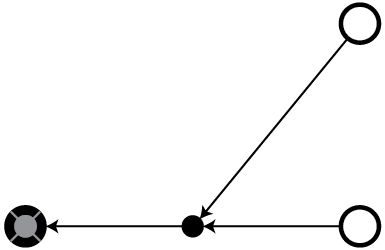
\includegraphics[width=\textwidth]{./img/method_experiment_merging}
		%!TEX root = ../report.tex

\begin{tikzpicture}
	\node[source, label={left:(100, 50)}, state, initial, initial text={}, initial where=above]			
		(c_0)						{$\mathbf{s_0}$};
	\node[source, label=below:{(100, -50)}, state, initial, initial text={}, initial where=right]		
		(c_1)	[below of=c_0] 		{$\mathbf{s_1}$};
	\node[vertex, label=below:{(0, -50)}, state]														
		(v_0) 	[left of=c_1]    	{$v_0$};
	\node[sink, label=below:{(-100, -50)}, state, accepting]										
		(k_0) 	[left of=v_0]		{$\mathbf{s_2}$};

	\path[->] (c_0) edge[edgeStyle] (v_0);
	\path[->] (v_0) edge[edgeStyle] (k_0);
	\path[->] (c_1) edge[edgeStyle] (v_0);
\end{tikzpicture}
		\caption{Merging traffic}
		\label{fig:method:experiment:merging}
	\end{subfigure}
	\begin{subfigure}{0.49\textwidth}
		\centering
		% 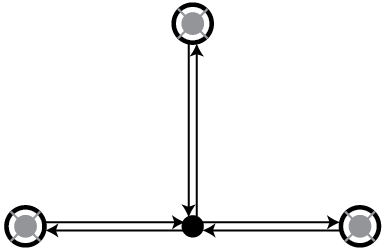
\includegraphics[width=\textwidth]{./img/method_experiment_intersection}
		%!TEX root = ../report.tex

\begin{tikzpicture}

	\node[label=left:{(0, 10)}, state, initial, initial text={}, initial where=above, accepting, source, sink]		
		(s_0)						{$s_0$};
	\node[vertex, label=below:{(0, -10)}, state]														
		(v_0) 	[below of=s_0]    	{$v_0$};
	\node[label=below:{(10, -10)}, state, initial, initial text={}, initial where=right, accepting, source, sink]		
		(s_1)	[right of=v_0] 		{$s_1$};
	\node[label=below:{(-10, -10)}, state, initial, initial text={}, initial where=left, accepting, source, sink]	
		(s_2)	[left of=v_0] 		{$s_2$};

	\path[->] (s_0) edge[edgeStyle] (v_0);
	\path[->] (v_0) edge[edgeStyle] (s_0);

	\path[->] (s_1) edge[edgeStyle] (v_0);
	\path[->] (v_0) edge[edgeStyle] (s_1);	

	\path[->] (s_2) edge[edgeStyle] (v_0);
	\path[->] (v_0) edge[edgeStyle] (s_2);		
\end{tikzpicture}
		\caption{Intersecting traffic}
		\label{fig:method:experiment:intersection}
	\end{subfigure}	
	% \caption{The graphs representing the network of streets used in our experiment, \subref{fig:method:experiment:merging} shows a graph that forces traffic to merge into a different lane with traffic, \subref{fig:method:experiment:intersection} presents a graph that forces cars to cross other traffic. In these graphs solid black circles indicate `normal' vertices, white circles with a black border are sources and the grey crossed out circles denote sinks.}
	\caption{The graphs representing the network of streets used in our experiment, \subref{fig:method:experiment:merging} shows a graph that forces traffic to merge into a different lane with traffic, \subref{fig:method:experiment:intersection} presents a graph that forces cars to cross other traffic. In these graphs filled vertices with a double border indicate sinks. A thick arrow indicates sources, which have a red border. Associated with each node is a location in the simulation space and a name.}
	\label{fig:method:experimentGraphs}
\end{figure}

\subsubsection{Measures}
\label{ss:method:experiment:measures}
We measure how long it takes a car to get from its source to its destination. Since we know the distance between all sources and destinations, we can compute the average speed of the car on its route. Although this average speed can hide some fluctuations it is a reasonable indicator in our case since each route has exactly one obstacle that can influence the time needed to traverse it. 